\documentclass{article}

% Imports
\usepackage{longtable}
\usepackage{indentfirst}
\usepackage{enumitem}
\usepackage{hyperref} %Hyperlinks
\usepackage{titlesec}
\usepackage{graphicx}
\usepackage{cleveref}
\usepackage[a4paper, total={6in, 9in}]{geometry}
\usepackage{minted}

\begin{document}

\begin{titlepage}
  \vspace*{1cm}

  \begin{center}
    {\Huge{Sistemas Operativos: Resumen}}
  \end{center}

  \vspace{0.4cm}

  \begin{center}
    {\LARGE{Facultad de Ingeniería de la Universidad de Buenos Aires}}\\
    \vspace{0.3cm}
    {\Large{Cátedra Mendez}}\\
    \vspace{0.3cm}
    {\large{2C 2023}}\\
  \end{center}

  \begin{center}
    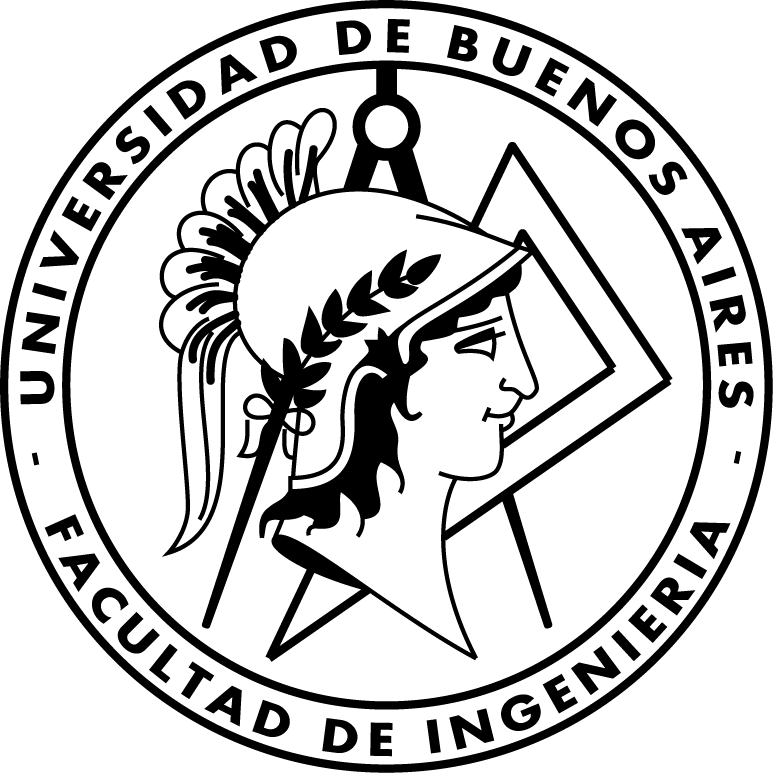
\includegraphics[scale=0.8]{media/Logo-fiuba.png}
  \end{center}
  \hspace*{-2cm}                                                           
    
\includegraphics[width=7cm]{media/GNU.png}
  \hspace*{3cm}                                                           
  \hspace{2.8cm}
    
\includegraphics[width=6cm]{media/Tux.png}
  \begin{center}
    
\includegraphics[width=6cm]{media/Larry.png}
  \end{center}

\end{titlepage}

\tableofcontents


\section{Programa}\label{programa}

Un programa es un archivo que posee toda la información de cómo
construir un proceso en memoria.

\begin{itemize}
\item
  Instrucciones de Lenguaje de Máquina: Almacena el código del algoritmo
  del programa.
\item
  Dirección del Punto de Entrada del Programa: Identifica la dirección
  de la instrucción con la cual la ejecución del programa debe iniciar.
\item
  Datos: El programa contiene valores de los datos con los cuales se
  deben inicializar variables, valores de constantes y de literales
  utilizadas en el programa.
\item
  Símbolos y Tablas de Realocación: Describe la ubicación y los nombres
  de las funciones y variables de todo el programa, así como otra
  información que es utilizada por ejemplo para debug.
\item
  Bibliotecas Compartidas: describe los nombres de las bibliotecas
  compartidas que son utilizadas por el programa en tiempo de ejecución
  así como también la ruta del linker dinámico que debe ser usado para
  cargar dicha biblioteca.
\item
  Otra información: El programa contiene además otra información
  necesaria para terminar de construir el proceso en memoria.
\end{itemize}

\section{Proceso}\label{proceso}

Proceso: Un archivo con información para generar el programa en memoria.
Tiene las instrucciones en assembler, punto de partida, datos, símbolos
y tabla de realocalizacion, etc\ldots{} Toda esta metadata, es la mitad
de los datos necesarios para lograr que el archivo se ejecute
(convirtiéndose así en un proceso), la otra mitad la hace el kernel.

Un Proceso es una entidad abstracta, definida por el Kernel, en la cual
los recursos del sistema son asignados

El kernel almacena la lista de procesos en una lista circular doblemente
enlazada llamada task list.

\subsection{Pasos en la creación de un
proceso}\label{pasos-en-la-creaciuxf3n-de-un-proceso}

\begin{enumerate}
\def\labelenumi{\arabic{enumi}.}
\item
  El kernel carga las instrucciones en memoria. Hay distintas partes del
  archivo que corresponden a distintos componentes.

  \begin{enumerate}
  \def\labelenumii{\alph{enumii}.}
  \item
    .text: Codigo
  \item
    .dato: variables globales
  \item
    .heap
  \item
    .stack
  \end{enumerate}
\item
  Crea el stack y el heap
\item
  Transfiere el control al programa actual
\item
  Protege al SO y al programa
\end{enumerate}

Cada proceso viene acompañado de varias abstracciones que el SO brinda
para la ejecución correcta del programa. Las abstracciones habituales
son: La memoria, el cpu, file descriptors, señales, etc.

Además, en el address space (posiciones de memoria al que pueden
acceder) del proceso, se incluye una porción del código del kernel. Este
incluye código que procesa la mayoría de syscalls (entre otras cosas).
Esto se hace para minimizar la cantidad de veces que se tiene que llamar
al ``verdadero'' kernel.

\subsection{Virtual memory}\label{virtual-memory}

Cada programa tiene un \textbf{address space propio.} El programa CREE
que tiene acceso a la totalidad de la memoria. Este mecanismo está
relacionado con el trabajo de ilusionista del sistema operativo.

En realidad, el SO mapea dicha memoria virtual a un espacio de la
memoria física.

\subsubsection{Mapeo de virtual a
fisica}\label{mapeo-de-virtual-a-fisica}

La traducción de memoria virtual a física es realizada por la MMU
(Memory management system) en conjunto con el sistema operativo. Esta
unidad de hardware se encarga de traducir direcciones virtuales a
direcciones físicas.

\subsection{Virtual processor}\label{virtual-processor}

De la misma manera que cada programa cree que tiene acceso total a la
memoria, pasa lo mismo con el procesador. Cada proceso cree que es el
único que usa el CPU.

Esto es hasta cierto punto ``verdadero''. Cuando el programa está siendo
ejecutado (en un momento determinado) SI es el único proceso que está
siendo ejecutado. Sin embargo, NO es el único proceso que accede al CPU
en el sistema. Como el cambio entre proceso y proceso es constante,
decimos que cada proceso tiene un \textbf{contexto}

\subsubsection{Contexto}\label{contexto}

Consiste en un conjunto de datos que un proceso tiene en un momento
determinado. Cuando se cambia de proceso a proceso, se da un
\textbf{context switch}: Se almacena el contexto de un proceso en
memoria y entra el nuevo proceso. Este proceso es \textbf{caro}. Es por
esto que se incluye parte del kernel en los procesos.

Hay muchos componentes que se guardan en el contexto:

\begin{itemize}
\item
  Nivel usuario
\item
  Nivel registro
\item
  Nivel Sistema
\end{itemize}

\subsection{\texorpdfstring{Estados }{Estados }}\label{estados}

Un proceso puede estar en varios estados. Los principales son: Running
(1 a la vez), ready (varios) y blocked (varios). El resto de los estados
posibles son variaciones de estos (también hay otros, pero esos son los
estados importantes).

\section{Kernel}\label{kernel}

\subsection{Punto de vista del
usuario}\label{punto-de-vista-del-usuario}

\begin{itemize}
\item
  El Sistema de Archivos o File System.

  \begin{itemize}
  \item
    Características:

    \begin{itemize}
    \item
      Estructura jerárquica
    \item
      Habilidad de crear y eliminar archivos
    \item
      Tratamiento de los dispositivos periféricos como si fueran
      archivos.
    \item
      protección de los archivos de datos
    \end{itemize}
  \end{itemize}
\item
  El Entorno de Procesamiento.

  \begin{itemize}
  \item
    El shell ejecuta los comandos buscando en ciertos directorios en una
    determinada secuencia.
  \item
    Dado que el shell es un programa no forma parte del Kernel del
    sistema operativo
  \end{itemize}
\item
  Los Bloques Primitivos de Construcción

  \begin{itemize}
  \item
    Proveer ciertos mecanismos para que los programadores construyan a
    partir de pequeños programas otros más complejos.
  \end{itemize}
\end{itemize}

\subsection{Cómo protege el kernel de un SO las aplicaciones y los
usuarios}\label{cuxf3mo-protege-el-kernel-de-un-so-las-aplicaciones-y-los-usuarios}

\begin{itemize}
\item
  Instrucciones Privilegiadas

  \begin{itemize}
  \item
    Distintos set de instrucciones para usar en distintos rings
  \end{itemize}
\item
  Protección de Memoria

  \begin{itemize}
  \item
    Dirección Virtual vs Dirección Física
  \item
    Espacio de direcciones
  \end{itemize}
\item
  Timer Interrupts

  \begin{itemize}
  \item
    Hardware Timer: cada timer interrumpe a un determinado procesador
    mediante una interrupción por hardware.
  \item
    Cuando una interrupción por tiempo se dispara se transfiere el
    control desde el proceso de usuario al Kernel
  \end{itemize}
\end{itemize}

\subsection{Cambio de contexto}\label{cambio-de-contexto}

\subsubsection{User Mode to Kernel Mode}\label{user-mode-to-kernel-mode}

\begin{itemize}
\item
  Interrupciones

  \begin{itemize}
  \item
    Señal asincrónica hacia el procesador avisando que algún evento
    externo requiere su atención
  \end{itemize}
\item
  Excepciones del Procesador

  \begin{itemize}
  \item
    Evento de hardware causado por una aplicación de usuario que causa
    la transferencia del control al Kernel.
  \end{itemize}
\item
  System Call

  \begin{itemize}
  \item
    Algún procedimiento provisto por el kernel que puede ser llamada
    desde el user level.
  \item
    Dado que todas las system calls son accedidas de la misma forma, el
    kernel tiene que saber identificarlas de alguna forma. Para poder
    hacer esto, la función wrapper \textbf{copia el número de la system
    call a un determinado registro de la CPU (\%eax).}
  \end{itemize}
\end{itemize}

\subsubsection{Kernel Mode to User Mode}\label{kernel-mode-to-user-mode}

\begin{itemize}
\item
  Nuevo Proceso
\item
  Continuar luego de una interrupción, excepción o una sys call
\item
  Cambiar entre diferentes procesos
\end{itemize}

\section{Signal}\label{signal}

Una signal (también llamadas interrupciones por software) es una
notificación que envía a un proceso cuando un determinado evento ocurre.

\begin{itemize}
\item
  Son análogas a las interrupciones por hardware, interrumpen el flujo
  normal de la ejecución de un programa, pero en la mayoría de los casos
  no es posible predecir el arribo de una señal.
\item
  Un proceso puede enviar una señal a otro proceso (se usa para
  sincronización).
\item
  Un proceso puede enviarse señales a él mismo.
\end{itemize}

Normalmente la fuente de envío de señales hacia un proceso es el Kernel.

\subsection{Motivos por los que el Kernel envía señales a un
proceso}\label{motivos-por-los-que-el-kernel-envuxeda-seuxf1ales-a-un-proceso}

\begin{itemize}
\item
  Una excepción de software (div por 0).
\item
  El usuario presiona algún carácter especial en la terminal (CRTL-C).
\item
  Un evento que tiene que ver con el software ocurrió, un proceso hijo
  terminó.
\end{itemize}

\subsection{Ciclo de vida de una
signal}\label{ciclo-de-vida-de-una-signal}

\begin{itemize}
\item
  Generada
\item
  Entregada
\item
  Pendiente
\end{itemize}

Una señal es generada por un evento, una vez generada, esta es entregada
a un determinado proceso, que tomará en algún momento una acción. El
tiempo entre la generación y la entrega de la señal está pendiente.

Una señal pendiente es entregada al proceso tan pronto como este esté
planificado para ser el próximo en correr o inmediatamente si este se
encuentra en ejecución.

A veces es necesario que un proceso no sea interrumpido por la entrega
de una señal. Para ello se agrega una máscara de señal.

Una vez que la señal se entrega, el proceso puede llevar a cabo una de
las siguientes acciones por defecto:

\begin{itemize}
\item
  La señal es ignorada: es descartada por el kernel y no tiene efecto
  sobre el proceso.
\item
  El proceso es terminado. Muchas veces se denomina abnormal process
  termination.
\item
  Un archivo de core dump es generado y el proceso terminado. (imagen de
  la memoria virtual)
\item
  El proceso es detenido: ejecución suspendida.
\item
  El proceso continúa su ejecución.
\end{itemize}

Un programa puede modificar la acción por defecto de una determinada
señal cuando ésta es entregada. Esto se denomina definir la
\textbf{disposition}

\subsection{Signal handler}\label{signal-handler}

Un signal handler es una función, escrita por el programador, que
realiza la tarea apropiada en respuesta a la entrega de una señal.

\section{Scheduling}\label{scheduling}

Es la parte del kernel que decide que se va a ejecutar y cuando.

\subsection{Conceptos relacionados}\label{conceptos-relacionados}

Multiplexación: Hacer que un recurso esté disponible para varios
procesos

Multiprogramación: La idea es que en la RAM haya varios programas
cargados en memoria (incluido el SO)

Time sharing: Consiste en establecer distintos intervalos de tiempo para
que distintos programas estén en el cpu

\subsection{Metricas}\label{metricas}

Para medir que tan bien anda un scheduler hay dos grandes métricas

\subsubsection{Turn around time}\label{turn-around-time}

``Tiempo que tarda una tarea en realizarse''

Se mide como:

(Tiempo en el que se completó una tarea) - (Tiempo en el que llegó la
tarea)

\subsubsection{Tiempo de respuesta}\label{tiempo-de-respuesta}

Mide que tan interactivo es un programa

Se mide como:

(Tiempo en el que inicia un programa) - (Tiempo llega una respuesta)

\subsection{Ejemplos de schedulers}\label{ejemplos-de-schedulers}

\subsubsection{FIFO}\label{fifo}

\begin{itemize}
\item
  Es un scheduler intuitivo.
\item
  Se procesan los procesos en el orden en el que llegaron.
\end{itemize}

Sufre de un gran problema, el \textbf{efecto convoy:} Si el primer
proceso es muy largo, te traba todo. Entonces, un proceso que es cortito
tiene que esperar un montón.

\paragraph{Shortest job first}\label{shortest-job-first}

Trata de mitigar el efecto convoy. Dice que si llegan dos procesos a la
vez, ejecuta el más corto primero.

Sin embargo, ES RARO que lleguen dos procesos A LA VEZ.

\paragraph{Shortest time to
completion}\label{shortest-time-to-completion}

Consiste en que siempre hace el proceso más corto. Si llega un proceso
más corto, para el que está haciendo y hace el que llega.

Sin embargo, esto presupone que el scheduler sabe la longitud del
proceso. Esto no suele ser el caso (no pasa).

\subsubsection{Round robin}\label{round-robin}

\begin{itemize}
\item
  Se define un time slice (unidad de tiempo fija).
\item
  Después de cada time slice ejecutas un nuevo proceso. Y va cambiando
  uno a uno en ``círculos''.
\end{itemize}

Esto logra un tiempo de respuesta mayor, dando lugar a más
``interactividad''. Pero viene al costo de \textbf{turn around time}:
Este cambio constante no es muy performante ya que hay un cambio de
contexto constante.

\subsubsection{Multi Level Feedback
Queue}\label{multi-level-feedback-queue}

\begin{itemize}
\item
  Trata de maximizar turn around time y tiempo de respuesta.
\item
  Consiste de muchas colas con prioridades distintas.
\item
  Cada tarea está en una única cola en un momento determinado.
\item
  Solo se procesan los procesos que están en la cola de más alta
  prioridad.

  \begin{itemize}
  \item
    Si hay varios procesos en más de una cola se realiza
    \hyperref[round-robin]{\underline{Round robin}}
  \end{itemize}
\end{itemize}

\paragraph{Asignación de
prioridades}\label{asignaciuxf3n-de-prioridades}

\begin{enumerate}
\def\labelenumi{\arabic{enumi}.}
\item
  Siempre que llega un proceso se le da la prioridad más alta
\item
  Si una tarea usa el CPU durante todo su timeslice entonces se le baja
  la prioridad
\item
  Si un tarea renuncia al cpu durante su time slice su prioridad aumenta
\end{enumerate}

Si un proceso usa el CPU durante TODO su timeslice significa que es un
proceso que es muy intenso y no es muy interactivo.\\
En cambio, en un proceso que rechaza el CPU, significa que no es un
proceso muy intenso y que es interactivo.

\paragraph{Problemas}\label{problemas}

\begin{itemize}
\item
  Starvation

  \begin{itemize}
  \item
    Problema: Los procesos que son muy heavies en cpu no son procesados
    nunca si hay procesos interactivos constantemente.
  \item
    Solución: Se implementa un \textbf{boost}, el cual implica que cada
    cierto periodo S, todos los procesos pasan a la mayor prioridad
  \end{itemize}
\item
  Gaming (de Gaming the system):

  \begin{itemize}
  \item
    Problema: Si un proceso es inteligente, podría, voluntariamente,
    dejar de pedir CPU para mantenerse siempre en la mayor prioridad
  \item
    Solución: Se implementa \textbf{accounting.} Se lleva una cuenta de
    cuantos time slices un proceso tuvo arriba del todo. Cuando llega a
    su cuota máxima, se tira para abajo
  \end{itemize}
\end{itemize}

\subsubsection{Completely Fair
Scheduler}\label{completely-fair-scheduler}

\begin{itemize}
\item
  Es el scheduler usado hoy en día en Linux.
\item
  Se basa en calcular proporciones de tiempo del procesador en vez de
  pensar en time slices de la misma longitud.
\item
  Es altamente escalable ya que usa estructuras de datos muy
  performantes.
\item
  Usa el concepto de virtual runtime.
\end{itemize}

Virtual runtime: Este es el runtime (tiempo que estuvo en el
procesador), normalizado por la cantidad de procesos runnable. Cuando
tiene que cambiar de proceso en ejecución, elegiría \textbf{el proceso
con menos vruntime para que sea el próximo en ser ejecutado.}

\paragraph{Parametros}\label{parametros}

\begin{itemize}
\item
  \textbf{Sched\_latency:}

  \begin{itemize}
  \item
    Mide la cantidad de tiempo antes del switcheo de proceso.
  \item
    Es dinámico y cambia con la cantidad de procesos.

    \begin{itemize}
    \item
      Problema: Si hay muchos procesos el cambio de contexto sería muy a
      menudo y habría una menor performance
    \item
      Solución: \textbf{min\_granularity}
    \end{itemize}
  \end{itemize}
\item
  \textbf{Min\_granularity:}

  \begin{itemize}
  \item
    Es una medida que define la MÍNIMA cantidad de tiempo que un time
    slice puede durar.
  \item
    Este valor es modificable. Por defecto vale 6ms
  \end{itemize}
\item
  \textbf{Niceness:}

  \begin{itemize}
  \item
    Mide la prioridad de un proceso.
  \item
    Va de -20 (mayor) a +19 (menor prioridad). Por defecto es 0.
  \item
    Cada valor de nice mapea a un \textbf{weight}
  \end{itemize}
\item
  \textbf{Time slice}:

  \begin{itemize}
  \item
    En CFS, es variable y se calcula así:

    \begin{itemize}
    \item
      \(time\ slice\  = \ \frac{weight_{k}}{\sum_{0}^{n - 1}weight} \cdot \ sched\ latency\)
    \item
      En espanol'': Su peso normalizado por el sched latency
    \end{itemize}
  \end{itemize}
\end{itemize}

\paragraph{Arbol rojo y negro}\label{arbol-rojo-y-negro}

Un árbol rojo-negro es un árbol binario de búsqueda en el que cada nodo
tiene un atributo de color cuyo valor es rojo o negro. En adelante, se
dice que un nodo es rojo o negro haciendo referencia a dicho atributo.

Además de los requisitos impuestos a los árboles binarios de búsqueda
convencionales, se deben satisfacer las siguientes reglas para tener un
árbol rojo-negro válido:

\begin{itemize}
\item
  Todo nodo es o bien rojo o bien negro.
\item
  La raíz es negra.
\item
  Todas las hojas (NULL) son negras.
\item
  Todo nodo rojo debe tener dos nodos hijos negros.
\item
  Cada camino desde un nodo dado a sus hojas descendientes contiene el
  mismo número de nodos negros.
\end{itemize}

Cuando el scheduler es invocado para correr un nuevo proceso, la forma
en que el scheduler actúa es la siguiente:

\begin{enumerate}
\def\labelenumi{\arabic{enumi}.}
\item
  El nodo más a la izquierda del árbol de planificación es elegido (ya
  que tiene el tiempo de ejecución más bajo), y es enviado a ejecutarse.
\item
  Si el proceso simplemente completa su ejecución, este es eliminado del
  sistema y del árbol de planificación.
\item
  Si el proceso alcanza su máximo tiempo de ejecución o de otra forma se
  para la ejecución del mismo voluntariamente o vía una interrupción)
  este es reinsertado en el árbol de planificación basado en su nuevo
  tiempo de ejecución (vruntime).
\item
  El nuevo nodo que se encuentre más a la izquierda del árbol será ahora
  el seleccionado, repitiéndose así la iteración.
\end{enumerate}

\section{Memoria}\label{memoria}

Espacio de direcciones: Representa el sandbox donde se aloja cada
proceso.

\subsection{Virtualización de
memoria}\label{virtualizaciuxf3n-de-memoria}

Mapeo de n elementos virtuales a m elementos físicos. Ningún proceso
sabe que la memoria está virtualizada.

La \textbf{virtual address} tiene que ser traducida a la
\textbf{physical address} por la MMU. El SO delega esa responsabilidad a
la MMU.

\subsubsection{Trabajo del SO}\label{trabajo-del-so}

El sistema operativo se encarga de manejar las direcciones de memoria
para minimizar la fragmentación y ser eficiente en tiempo.

El sistema operativo tiene que involucrarse en los puntos claves de la
address translation para:

\begin{itemize}
\item
  Setear al hardware de forma correcta para que esta traducción se de
  lugar;
\item
  Gerenciar la memoria

  \begin{itemize}
  \item
    Manteniendo registro de qué parte está libre.
  \item
    Qué parte está en uso.
  \item
    Manteniendo el control de la forma en la cual la memoria está siendo
    utilizada.
  \end{itemize}
\item
  Intervenir de forma criteriosa como mantener el control sobre toda la
  memoria usada.
\end{itemize}

\subsection{Implementaciones}\label{implementaciones}

\subsubsection{Segmentacion/ Base +
Bound}\label{segmentacion-base-bound}

\begin{itemize}
\item
  Cada proceso tiene su propio address space.

  \begin{itemize}
  \item
    Address space: contiene todo el estado de la memoria de un programa
    en ejecución.
  \end{itemize}
\item
  Los límites de ese address space están delimitados por dos registros.
  \textbf{Base \& Bound}.

  \begin{itemize}
  \item
    Base contiene la dirección inicial del address space
  \item
    Bound tiene el tamaño del address space o el límite del mismo.
  \end{itemize}
\end{itemize}

Para traducir de la dirección virtual a la física se usa la cuenta:\\
Registro\textsubscript{base} + offset.

Si eso daba mayor al bound, entonces tenías un error (estás tratando de
acceder a memoria que no le pertenece al proceso.)

\paragraph{En x86}\label{en-x86}

En x86 había más de dos registros para la segmentación, hay 4. CS (code
segment), DS (data segment), SS (stack segment), ES (Extra segment).
Cada uno de esos registros tiene su propio offset. 2 bits de dirección y
los otros 30 de offset (La longitud de cada dirección es la longitud de
la arquitectura, en x86 es 32 bits).

El SO se encarga de que las direcciones virtuales no mapeen a lago por
fuera. El error ``Segmentation fault'' se daba justamente cuando
tratabas de acceder a memoria por fuera de tu segmento.

La segmentación permitía tener procesos mezclados en memoria. Nos es
como el base and bound tradicional en donde había un único ``bloque''.

\subsubsection{Memoria paginada}\label{memoria-paginada}

\begin{itemize}
\item
  Se divide la memoria física y virtual.
\item
  La memoria virtual está dividida en \textbf{pages} y la física en
  \textbf{frames.}

  \begin{itemize}
  \item
    Cada frame, mide lo mismo que cada page que mide lo mismo que 1k.
  \end{itemize}
\item
  Se mapea cada frame a cada pagina.
\item
  La virtual address está partida en 3 sectores.
\end{itemize}


% Mas pixelada esta foto imposible jajajaj
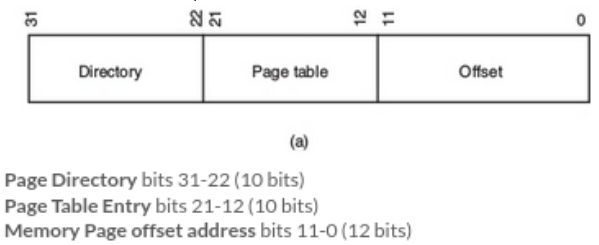
\includegraphics[width=6.20704in,height=2.52044in]{media/MemoriaPaginada.png}

\paragraph{\texorpdfstring{Page directory
}{Page directory }}\label{page-directory}

\begin{itemize}
\item
  Esta primera sección apunta a una tabla llamada La \textbf{Page
  Directory.}
\item
  Esta tabla tiene elementos de 4 bytes (32 bits). Tiene 1024 entradas
  (de 0 a 1023). La tabla en total mide 4096 bytes.
\item
  \textbf{Cada elemento apunta a OTRA tabla.} Es decir, que tenes 1024
  entradas a 1024 tablas. Vamos a decir que guarda la dirección de la
  \underline{tabla B.}
\item
  Cada tabla tiene 4mb de almacenamiento. Si el proceso requiere de más
  memoria, se le asigna otra tabla.
\item
  De los 32 bits de la entrada en la page directory, solo son los
  primeros 20 que apuntan a la otra tabla. Los otros 12 se usan para
  metadata de la tabla en cuestión.
\end{itemize}

\paragraph{Page Table Entry}\label{page-table-entry}

\begin{itemize}
\item
  En estos 10 bits, está \textbf{EN QUE POSICIÓN} de la \underline{tabla B}
  fijarte.
\item
  Entonces vos tenes la dirección de la tabla b (que lo obtuviste
  arriba) + la dirección en la que te tenes que fijar.
\item
  Esa dirección es el \textbf{frame} en el que tenes la memoria deseada
\end{itemize}

\paragraph{Memory page offset}\label{memory-page-offset}

\begin{itemize}
\item
  Indica el offset de la página.
\end{itemize}

Este esquema provee una granularidad mucho mayor. Hay un registro (CR3)
que guarda la dirección de la page directory de cada proceso.

\section{Cache}\label{cache}

TODO: Copiar \footnote{\label{notaTaller}Esto no lo esta resumido porque justo lo vimos en taller; y el concepto es el mismo que en taller. Si tenes resumido esto, los PR son mas que bienvenidos: PONERLINK}

\section{Threads}\label{threads}
 TODO: Copiar \footnote{Ver \cref{notaTaller}}


\section{Filesystem}\label{filesystem}

Forma de organizar los datos de forma persistente.

Un dato es persistente cuando está almacenado hasta que es borrado (la
ram no aplica

porque se borra cuando se le corta la corriente).

A nivel SO es una abstracción que provee datos con un nombre.

Contiene:

\begin{itemize}
\item
  Archivos: Contienen información
\item
  Directorios: Contenedor de archivos y otros directorios.
\end{itemize}

\section{Unix filesystem hierarchy}

En Unix hay un estándar de directorios. Esto quiere decir que hay
directorios que contienen archivos con un propósito común. Ejemplos:

\begin{itemize}
\item
  /dev: Dispositivos
\item
  /etc: Archivos de configuración
\item
  /proc: Metadata sobre los procesos, como fd, etc
\item
  /lib: Bibliotecas.
\item
  /bin: Binarios genericos.
\item
  /sbin: Binarios relacionados con el mantenimiento del sistema
\item
  /usr: Un montoooon de cosas. Hoy en dia, la mayoria de las distros, guardan los binarios de /bin y /sbin aca.
\item
  /mnt: Directorio para montar dispositivos externos (USB, Harddrives, etc) 
\item
  /boot: Archivos necesarios para el booteo
\item
  /sys: Tiene archivos ``virtuales'' que contienen información del kernel.
\item
  /tmp: Archivos temporales
\item
  /root: Directorio ``HOME'' de root. Cuando root se logea, se logea aca.
\item
  /home: Aca estan los directorios de los distintos usuarios
\end{itemize}

Etc, hay mas y pueden variar. Es solo un estandar.

\subsection{Virtual filesystem}\label{virtual-filesystem}

Subsistema del kernel que estandariza el procesado y tratamiento de
archivos de todos los filesystems posibles.

Este hace de interfaz para poder realizar operaciones intra filesystems
distintos.

Cuando interactúa con el SO, uno simplemente llama a las syscalls
``tradicionales'': open, close, write. Es el virtual filesystem el que
se encarga de hacer la llamada a la función correspondiente.

-\textgreater{} write() -\textgreater{} sys\_write() -\textgreater{}
write específico al filesystem (ejemplo write\_xfs) -\textgreater{}
escribir al disco.

\subsubsection{Objetos del filesystem}\label{objetos-del-filesystem}

Una implementación de filesystem necesita de estas cosas para ser
considerado un vfs:

\begin{itemize}
\item
  Super bloque: Representa en file system en sí mismo.
\item
  Inodo: Representa un archivo en el sistema.
\item
  Dentry: Un conjunto de entradas en un directorio. Cada una de estas
  representa los archivos presentes en el directorio.
\item
  File: Representación de un archivo en memoria utilizado por un
  proceso.
\end{itemize}

Contenido de archivo

\begin{itemize}
\item
  Metadata: información acerca del archivo que es comprendida por el
  Sistema Operativo, esta información es :

  \begin{itemize}
  \item
    Tamaño
  \item
    fecha de modificación
  \item
    Propietario
  \item
    información de seguridad (que se puede hacer con el archivo.
  \end{itemize}
\item
  Datos: son los datos propiamente dichos que quieren ser almacenados.
  Desde el punto de vista del Sistema Operativo, un archivo o file no es
  más que un arreglo de bytes sin tipo.
\end{itemize}

\subsection{Implementación de
filesystem}\label{implementaciuxf3n-de-filesystem}

Filesystem, refiere a dos cosas. Al \textbf{concepto} del filesystem y
la \textbf{implementación}.\\
Hay muchas implementaciones del ``filesystem''. Cada una funciona
``igual'' pero almacena metadata distinta y tiene algunos pros/contras.

\subsection{API del filesystem}\label{api-del-filesystem}

\subsubsection{API archivos}\label{api-archivos}

\paragraph{open}\label{open}

Devuelve el file descriptor del archivo abierto

\paragraph{creat}\label{creat}

Crea un archivo y devuelve la el file descriptor

\paragraph{close}\label{close}

Le pasas un file descriptor y lo cierra

\paragraph{read}\label{read}

Trata de leer count bytes del fd y los guarda en el buffer. Devuelve la
cantidad de bytes leidos.

\paragraph{write}\label{write}

Trata de escribir count bytes del fd y los guarda en el buffer. Devuelve
la cantidad de bytes escritos.

\paragraph{lseek}\label{lseek}

Sobre escribe el offset de un file descriptor.

\paragraph{dup}\label{dup}

Duplica un fd, devolviendo el numero mas chico disponible

\paragraph{dup2}\label{dup2}

Duplica un fd, el que vos le especificas

\paragraph{link}\label{link}

Crea un hard link.

\paragraph{unlink}\label{unlink}

Elimia un nombre de un archivo del filesystem.

Si además ese nombre era el último nombre o link del archivo y no hay
nadie que tenga el archivo abierto lo borra completamente del sistema de
archivos.

\subsubsection{API directorios}\label{api-directorios}

\paragraph{\texorpdfstring{mkdir }{mkdir }}\label{mkdir}

Crea un directorio

\paragraph{\texorpdfstring{rmdir }{rmdir }}\label{rmdir}

Borra un directorio

\paragraph{opendir}\label{opendir}

Abre y devuelve un stream que corresponde al directorio que se está
leyendo.

Devuelve un DIR * (steam que representa e ldirectorio que se está
leyendo)

\paragraph{readdir}\label{readdir}

Lee un DIR * y devuelve unn dirent *

El dirent tiene el nombre del archivo y un inodo

\paragraph{closedir}\label{closedir}

Dada un close DIR*, lo cierra

\subsubsection{API metadatos}\label{api-metadatos}

\paragraph{stat}\label{stat}

Dado un pathname, devuelve estadisticas sobre el archivo

Devuelve un struct stat

\paragraph{access}\label{access}

Dado un pathname, dice si un proceso tiene permiso a usar el archivo de
una manera expecica.

Le podes preguntar si existe, lo podes leer, escribir o ejecutar.

\paragraph{chmod}\label{chmod}

Dado un pathname y un modo, le cambia los bits del modo de acceso.

\paragraph{chown}\label{chown}

Dado un pathname, puede cambiar el owner (user y o group)

\subsubsection{Ejemplos}\label{ejemplos}

\paragraph{ls}\label{ls}


\begin{minted}{c}
  int main() {
    DIR *dp;
    struct dirent *ep;

    dp = opendir("./");
    if (dp != NULL) {

        while (ep = readdir (dp))
            puts(ep->d_name);

        (void) closedir(dp);
    } else {
        perror ("Couldn't open the directory");
    }

    return 0;
  }
\end{minted}
% \begin{longtable}[]{@{}
%   >{\raggedright\arraybackslash}p{(\columnwidth - 0\tabcolsep) * \real{1.0000}}@{}}
% \toprule\noalign{}
% \begin{minipage}[b]{\linewidth}\raggedright
% int main() \{\\
% DIR *dp;\\
% struct dirent *ep;\\
% \strut \\
% dp = opendir("./");\\
% if (dp != NULL) \{\\
% while (ep = readdir (dp))\\
% puts(ep-\textgreater d\_name);\\
% (void) closedir(dp);\\
% \}\\
% else\\
% perror ("Couldn\textquotesingle t open the directory");\\
% \strut \\
% return 0;\\
% \}\strut
% \end{minipage} \\
% \midrule\noalign{}
% \endhead
% \bottomrule\noalign{}
% \endlastfoot
% \end{longtable}

\subsection{File descriptors y
archivos}\label{file-descriptors-y-archivos}

No hay una correspondencia 1 a 1 entre archivos e inodos. A veces, es
muy útil y necesario tener varios file descriptors referenciando al
mismo archivo abierto.

Por esto existen mecanismos en el kernel para esto:

\begin{itemize}
\item
  Per process file descriptor table
\item
  System wide file descriptor table

  \begin{itemize}
  \item
    El offset actual del archivo (que se modifica por read(), write() o
    por lseek();
  \item
    los flags de estado que se especificaron en la apertura del archivo
    ( los flags arguments de open());
  \item
    el modo de acceso (solo lectura,solo escritura, escritura-lectura);
  \item
    una referencia al objeto i-nodo para este archivo.
  \end{itemize}
\item
  File system inode table
\end{itemize}

\subsection{Very simple filesystem}\label{very-simple-filesystem}

Ejemplo de implementación de filesystem.

La unidad básica es el bloque. Tiene 4k de bytes de tamaño cada bloque.

\subsubsection{Division data y metadata}\label{division-data-y-metadata}

Como sabemos cuanto dedicarla al almacenamiento de datos y cuánto darle
al almacenamiento de metadatos?

Tenes que saber cuantos inodos vas a tener en el filesystem.

Fórmula para cantidad de inodos en un bloque = Tamaño bloque / tamaño
inodo (256).

La suposición inicial es que como mínimo un archivo ocupa un bloque.

Sin embargo, no podes usar todo el disco para inodos. Necesitas espacio
para la metadata.

\paragraph{Super bloque}\label{super-bloque}

El VFS tiene una referencia a este superbloque.

Contiene "toda" la información del sistema de archivos. Además, tiene
una tabla donde se encuentran los inodos. Sabe dónde empiezan los
bloques de inodo y, a través de un offset, puede encontrar el resto

\paragraph{Bloque de Bitmap de bloques y bloque bitmap de
inodos}\label{bloque-de-bitmap-de-bloques-y-bloque-bitmap-de-inodos}

Tienes que saber qué bloques están ocupados y que inodos están ocupados.

Para esto se usa un bitmap. En 32 bit, podes mapear hasta 32768 inodos y
bloques.

Si tuvieses un disco con más espacio necesitarías más bloques.

\paragraph{Bloques de metadatos}\label{bloques-de-metadatos}

La cantidad de bloques de metadatos necesarios se calcula de la
siguiente manera:

\# bloques / 16

Ya que en cada bloque entran 16 inodos

\paragraph{Bloques de datos}\label{bloques-de-datos}

El resto de los bloques libres es el espacio que se utilizará para los
datos.

\paragraph{Inodo}\label{inodo}

Contiene información sobre el archivo.

\begin{itemize}
\item
  4 bits que te indica qué tipo de archivo es
\item
  Link count (cantidad de hard links)
\item
  User ID y el group de user
\item
  Sticky bit
\item
  3 bits para el permiso de usuario
\item
  3 bits para el permiso de grupo
\item
  3 bits para el permiso de otros
\item
  Punteros a bloques (en el VSFS).

  \begin{itemize}
  \item
    Guarda punteros a bloques.
  \item
    Esto te permite que los bloques del archivo puedan estar esparcidos
    en el discos.
  \item
    Si es más grande, el bloque 13 guarda un puntero a un bloque con
    punteros a bloques.
  \item
    Si es mas grande, el bloque 14 apunte a un bloque que apunta a
    bloques que apunta a bloques (con esto podes tener un archivo de
    *4TB*).
  \item
    Si tenes uno mas grande todavia tenes un puntero de 3ple
    indirección.
  \end{itemize}
\end{itemize}

\section{Booteo}\label{booteo}

Este proceso es denominado bootstrap, y generalmente depende del
hardware de la computadora. En él se realizan los chequeos de hardware y
se carga el bootloader, que es el programa encargado de cargar el Kernel
del Sistema Operativo. Este proceso consta de 4 partes.

\subsection{Memoria}\label{memoria-1}

Distintas partes de la memoria (en 32 bits) tienen distintos propósitos.

\begin{itemize}
\item
  Low memory: 0 hasta 640KB
\item
  VGA: 640 a 768
\item
  Low memory: 768 y 960
\item
  BIOS ROM: 960KB a 1M
\end{itemize}

\subsection{Modo de la CPU}\label{modo-de-la-cpu}

\begin{itemize}
\item
  Real: Direcciones de 16 bits. Todas fisicas
\item
  Protegido: Direcciones de 32 bit. Fisicas
\end{itemize}

\subsection{Boot}\label{boot}

Proceso que lleva varios pasos

\begin{enumerate}
\def\labelenumi{\arabic{enumi}.}
\item
  Bios:

  \begin{enumerate}
  \def\labelenumii{\alph{enumii}.}
  \item
    Arranca en modo real
  \item
    Cuando prendes la máquina, se lee de la parte ROM de la memoria.
  \item
    Detecta un disco booteable y lo trata de meter en memoria.
  \item
    Lee del disco los primeros 512 bytes. Esos 512 bytes son el
    bootloader. No más no menos.
  \item
    0000-7C00
  \item
    En 7C00 esta es la primera instrucción que se ejecuta (apunta el
    EIP).
  \end{enumerate}
\item
  Bootloader

  \begin{enumerate}
  \def\labelenumii{\alph{enumii}.}
  \item
    Inicializa el stack segment, data y extra
  \item
    Enciende el modo protegido, lo cual saca el modo real y habilita las
    instrucciones de 32 bits.
  \item
    Una vez hecho eso pone en el esp el main del boot.
  \end{enumerate}
\item
  Bootloader en C

  \begin{enumerate}
  \def\labelenumii{\alph{enumii}.}
  \item
    Lee el encabezado del ELF. Chequea que el ELF tenga el valor mágico
    correcto.
  \item
    Busca todos los segmentos ejecutables del kernel y los carga en
    memoria.
  \item
    Después, llama al punto de entrada y ejecuta lo que está en memoria
    (aka la parte ejecutable del kernel).
  \end{enumerate}
\end{enumerate}

\section{Máquinas virtuales}\label{muxe1quinas-virtuales}

Es la virtualización de la totalidad de una computadora.

Definición: Entorno de computación completo. Con sus propias
capacidades. Aisladas una de las otras.

\subsection{Tipos Lenguaje}\label{tipos-lenguaje}

\subsubsection{Lenguaje}\label{lenguaje}

Ej: JVM

No las vamos a ver en clase. Fundamentalmente un intérprete.

\subsubsection{Liviana}\label{liviana}

Docker

El kernel es el que aísla cosas de otras.

\subsubsection{De sistema}\label{de-sistema}

Queres tener sobre el mismo hardware varios sistemas operativos.

\paragraph{Virtual machine monitor}\label{virtual-machine-monitor}

Es el que se encarga de sincronizar las distintas máquinas virtuales.

\subsection{Utilidades}\label{utilidades}

\begin{itemize}
\item
  Diversidad: Una sola máquina, varios so.
\item
  Consolidación de servidores: Aislar distintos servicios. Es la forma
  más fuerte de aislamiento
\item
  Aprovisionamiento rápido: Crear una máquina virtual es trivial. Antes
  tenía que tener el hardware para correr tus programas.
\item
  Alta disponibilidad: SI tenes que matar una máquina hardware lo podes
  hacer fácilmente, moves la máquina virtual a otra nueva
\item
  Seguridad: Más aisladas y más fácilmente monitoreable
\item
  Scheduling de recursos compartidos
\item
  Cloud computing: Se basa en las máquinas virtuales.
\end{itemize}

\subsection{Requerimientos}\label{requerimientos}

\begin{itemize}
\item
  Fidelidad

  \begin{itemize}
  \item
    Es equivalente al hardware real. El SO debería pensar que está
    corriendo en un hardware real.
  \item
    Tiene que ser totalmente transparente.
  \end{itemize}
\item
  Seguridad

  \begin{itemize}
  \item
    Tiene que estar aisladas una de las otras
  \end{itemize}
\item
  Eficiencia

  \begin{itemize}
  \item
    En el peor de los casos tiene que andar más lento
  \end{itemize}
\end{itemize}

\subsection{Tipos de VM}\label{tipos-de-vm}

\subsubsection{SO especial Hypervisor - Tipo
1}\label{so-especial-hypervisor---tipo-1}

Se encarga de supervisar las distintas vms. No hay SO base, solo el
hypervisor.

Tenías un SO especial/privilegiado para supervisar y configurar.

Conceptualmente similar a un microkernel.

\subsubsection{Hypervisor en espacio de usuario - Tipo
2}\label{hypervisor-en-espacio-de-usuario---tipo-2}

El supervisor es instalado como un programa más, corriendo en espacio de
usuario.

\subsection{Técnicas de
virtualización}\label{tuxe9cnicas-de-virtualizaciuxf3n}

Todas estas técnicas se usan de forma coordinada.

\begin{itemize}
\item
  Multiplexing: Tenes una única memoria física y la dividis en varias
  cosas virtuales
\item
  Aggregation: Varias cosas que hacen que se parezca como una.
\item
  Emulation: Emulas algo que no tenes con algo que tenes. Menos
  eficiente.
\end{itemize}

\subsection{Formas de implementar}\label{formas-de-implementar}

\subsubsection{Emular todo}\label{emular-todo}

\begin{itemize}
\item
  Emulas todo, el hipervisor no le da acceso a ninguna de los
  componentes reales al SO guest.
\item
  Esto no es particularmente eficiente. Si queres correr varios sistemas
  operativos se complica.
\end{itemize}

\paragraph{Qemu}\label{qemu}

\begin{itemize}
\item
  Tiene un JIT a un lenguaje intermedio.
\item
  Interpreta ese lenguaje en el momento.

  \begin{itemize}
  \item
    Eso es lo que permite que el qemu ejecute varias arquitecturas.
  \item
    Si la arquitectura es la misma, se saltea el proceso de traducción,
    se ejecuta directamente el código.
  \end{itemize}
\end{itemize}

\subsubsection{Ejecución directa}\label{ejecuciuxf3n-directa}

Las instrucciones de la máquina virtual se ejecutan directamente en el
cpu host.

Se complica si tenes varias máquinas que quieren ir al mismo hardware
(ej, disco rígido).

El VMM hace de scheduler entre las distintas vm del acceso.

La vm le pide al hypervisor, el hypervisor al SO y recién ahí.

Esto rompe la fidelidad, porque el SO tiene que saber pedirle al
hipervisor. No anda "asi nomas".

El protocolo de la syscall está definido. Pero no está definido el
protocolo para que el kernel le hable al hipervisor.

El truco es usar los discos no usados del cpu (ring 1,2, etc). Esto se
debe a que en el cpu cambia de ring en los General Protection Exception.
La VMM atrapa esta excepción. Esto se llama *trap and emulate*.

\paragraph{Hay problemas}\label{hay-problemas}

Intel añadió la instrucción popf que si se ejecuta sin los privilegios
correctos \textbf{NO} hay excepción.

Esto arruina toda la idea del trap and emulate. Si un SO huésped depende
de popf, estás jodido.

\paragraph{Soluciones}\label{soluciones}

\begin{itemize}
\item
  Traduccion binaria: Traducción en tiempo de ejecución de las
  instrucciones sensibles. El hipervisor tiene que ver que se está
  ejecutando y reemplazar las instrucciones truchas por buenas. Este
  comportamiento es como una emulación pero a menor escala. No se usa
  hoy en día. Muy difícil
\item
  Para virtualización: La guest sabe que es una vm. Llama a una system
  call que es atrapada por el hipervisor. Esto obvia el trucazo. Esto lo
  que tiene de malo, es que no funciona en cualquier sistema operativo.
  El so tiene que estar preparado para eso. Fácil para el hypervisor,
  jodido para el que implementa el so.
\item
  Virtualización asistida por hardware: Extensiones para el procesador.
  Añadieron un anillo adicional. Un anillo es el root mode y el non root
  mode es el anillo para las cosas virtualizadas. Si ejecutas popf en
  non root mode saltas al root mode.

  \begin{itemize}
  \item
    En el root mode kernel corre en el ring0 y el usermode en ring3
    (como siempre).
  \item
    En el non root mode kernel corre en el ring0 y el usermode en ring3
    (como siempre).
  \item
    El que puede poner algo en root mode o en un non root mode es el
    kernel.

    \begin{itemize}
    \item
      Hay instrucciones para esto vmlaunch. El vmexit es el inverso.
    \end{itemize}
  \end{itemize}
\item
  Virtualización moderna (KVM): Podes lanzar las vms como si fuesen
  procesos. Lanzas qemus que configuran usando la asistencia por
  hardware. Así, el scheduler del kernel schedulea las máquinas
  virtuales. El kernel es el que pasa de modo virtual a no virtual.
\end{itemize}

\subsubsection{Teorema de la VMM}\label{teorema-de-la-vmm}

Un VMM se puede construir si el conjunto de instrucciones sensibles es
un subconjunto de instrucciones privilegiadas

\textbf{Instrucciones sensibles}: Instrucciones que se ejecutan
diferente si están en modo usuario o kernel. Eg. I/O, modificar MMU, etc

\textbf{Instrucciones privilegiadas}: Instrucciones que causan traps en
modo usuario pero no en modo supervisor

\end{document}